% Compile twice with pdfLaTeX. Exactly 15 frames; no overlays or appendix frames.
% Scientific snapshot: 2671f6984b87f1d89613ba81d8b0e99798cd3f58.
% Archived results, not newly run synthesis experiments. See NOTES.md.
\documentclass[aspectratio=169,11pt]{beamer}
\usepackage[T1]{fontenc}
\usepackage{lmodern}
\usepackage{amsmath,amssymb,booktabs,array}
\usepackage{tikz,pgfplots}
\usetikzlibrary{arrows.meta,positioning}
\pgfplotsset{compat=1.18}
\definecolor{ink}{HTML}{183044}
\definecolor{accent}{HTML}{007C83}
\definecolor{muted}{HTML}{64727D}
\definecolor{pale}{HTML}{EDF4F5}
\definecolor{control}{HTML}{C98349}
\definecolor{equal}{HTML}{CBD3D8}
\setbeamercolor{normal text}{fg=ink,bg=white}
\setbeamercolor{frametitle}{fg=ink,bg=white}
\setbeamercolor{structure}{fg=accent}
\setbeamercolor{block title}{fg=accent,bg=pale}
\setbeamercolor{block body}{fg=ink,bg=pale}
\setbeamercolor{footline}{fg=muted,bg=white}
\setbeamerfont{frametitle}{size=\Large,series=\bfseries}
\setbeamersize{text margin left=7mm,text margin right=7mm}
\setbeamertemplate{navigation symbols}{}
\setbeamertemplate{frametitle}{\vspace{1mm}\insertframetitle\par\vspace{1mm}{\color{accent}\hrule}\vspace{1mm}}
\newcommand{\partnamebar}{Problem and learned search}
\setbeamertemplate{footline}{\hspace{7mm}\scriptsize\partnamebar\hfill\insertframenumber/15\hspace{7mm}\vspace{2mm}}
\setlength{\abovedisplayskip}{5pt}
\setlength{\belowdisplayskip}{5pt}
\newcommand{\ket}[1]{\lvert #1\rangle}
\newcommand{\bra}[1]{\langle #1\rvert}
\newcommand{\F}{\mathbb F_2}
\newcommand{\AND}{\operatorname{AND}_0}
\newcommand{\CX}{\operatorname{CNOT}}
\newcommand{\CZ}{\operatorname{CZ}}
\newcommand{\src}[1]{\par\vfill{\fontsize{6.6}{7.8}\selectfont\color{muted}#1\par}}
\newcommand{\takeaway}[1]{\par\smallskip\begin{beamercolorbox}[sep=1.6mm,wd=\linewidth]{block body}\small #1\end{beamercolorbox}}
\newcommand{\labeltext}[1]{{\color{accent}\bfseries #1}}
\title{Quantum Phase Oracles with Fewer Clean Ancillas}
\author{}
\date{}
\begin{document}

% ======================= PAGES 1--7 =======================
% 1
\begin{frame}[t]{1. The problem: implement a Boolean phase with few ancillas}
\small
A binary neural network (BNN) maps a finite input $z$ to an output. Let
\[
 p(z)=1\quad\Longleftrightarrow\quad\text{the output violates a specified property}.
\]
A phase oracle marks such inputs without measuring them:
\[
 O_p\ket z=(-1)^{p(z)}\ket z,
 \qquad \sum_z\alpha_z\ket z\ \longmapsto\ \sum_z\alpha_z(-1)^{p(z)}\ket z.
\]
With $A$ clean ancillas, put $J_A\ket z=\ket z\ket0^{\otimes A}$. A unitary implementation obeys
\[
 U_CJ_A=J_AO_p.
\]
\takeaway{Reduce the largest number of ancillas needed at once. Also report $T$ gates, CNOTs, total gates, and time. Every auxiliary qubit must return to $\ket0$.}
\src{Motivation: Nielsen--Chuang, Ch. 6 [NC]. The tested functions are structured feature-and-mask predicates, not complete BNN verification workloads [D].}
\end{frame}

% 2
\begin{frame}[t]{2. Why a cheaper oracle matters for amplitude amplification}
\small
Start with $\ket\psi=2^{-n/2}\sum_z\ket z$. If $M$ inputs violate the property, write
\[
 \ket\psi=\cos\theta\ket{\mathrm{safe}}+\sin\theta\ket{\mathrm{violating}},
 \qquad \sin^2\theta=M/2^n.
\]
For $0<M<2^n$, the two displayed states are normalized uniform sums over their sets.
\[
 Q=(2\ket\psi\bra\psi-I)O_p,
 \qquad \Pr[\mathrm{violation\ after\ }j\mathrm{\ steps}]
       =\sin^2((2j+1)\theta).
\]
\labeltext{Reason.} The oracle and the reflection about $\ket\psi$ are two reflections; their product rotates this two-dimensional state by $2\theta$.
\takeaway{Each amplification step calls the oracle again. A smaller oracle reduces this repeated cost. Not finding a violation in a finite run is not, by itself, a proof that none exists.}
\src{Standard amplitude-amplification construction [NC]. The reported resource counts later concern the oracle only: state preparation and the other reflection are excluded [D].}
\end{frame}

% 3
\begin{frame}[t]{3. A frontier record describes one partial quantum circuit}
\small
The frontier $\mathcal F_t$ contains discovered candidates that can still be extended. A coherent record is
\[
 \boxed{v=(G_v,\Theta_v,\mathcal R_v,\phi_v,\rho_v).}
\]
\begin{center}
\begin{tabular}{@{}ll@{}}
$G_v$ & The actual gates and their dependency graph.\\[2pt]
$\Theta_v$ & The Clifford transformation, stored as a tableau.\\[2pt]
$\mathcal R_v$ & An ordered sequence of Pauli rotations.\\[2pt]
$\phi_v$ & The scalar phase needed for exact equality.\\[2pt]
$\rho_v$ & Gates, per-wire depths, and other consumed resources.
\end{tabular}
\end{center}
\[
 U_v=e^{i\phi_v}C_vR_{P_m}(\theta_m)\cdots R_{P_1}(\theta_1)
 \qquad\text{(rightmost operator acts first).}
\]
\takeaway{The RL state $S_t$ is the whole search situation: frontier, recorded alternatives, and remaining limits. A single circuit record $v$ is an outer action, not the whole RL state.}
\src{Native circuit representation and frontier: branch files model.py and native\_search.py [N]. Measurement protocols need extra classical-outcome information; see slide 8.}
\end{frame}

% 4
\begin{frame}[t]{4. The tableau and rotations preserve exact quantum action}
\small
\begin{columns}[T,onlytextwidth]
\begin{column}{0.48\textwidth}
\labeltext{Clifford tableau}
\[
 C X_j C^\dagger,\quad C Z_j C^\dagger
\]
are signed Pauli operators. Their stored images specify how $C$ transports every Pauli, up to a scalar phase.

\smallskip
$H$, $S$, and CNOT are Clifford gates. The separate $\phi_v$ retains the required scalar phase.
\end{column}
\begin{column}{0.48\textwidth}
\labeltext{Ordered Pauli rotations}
\[
 R_P(\theta)=e^{-i\theta P/2},
 \quad P=\pm P_1\otimes\cdots\otimes P_n.
\]
Here each $P_j$ is $I,X,Y,$ or $Z$. In particular,
\[
 T=e^{i\pi/8}R_Z(\pi/4).
\]
Noncommuting rotations cannot in general be exchanged. Their order is retained.
\end{column}
\end{columns}
\smallskip
\labeltext{Dependency graph.} A gate on wires $Q_g$ ends at layer
\[
 d(g)=1+\max_{q\in Q_g} d_q;
 \qquad d_q\leftarrow d(g)\ \ (q\in Q_g).
\]
It therefore records both the circuit and which operations may overlap. Exact rewrites identify equal operators; their actual gate costs remain separate.
\src{Clifford and Pauli facts: [NC]. Exact scalar handling, ordered rotations, and per-wire dependency updates: [N]. Policies use small numerical summaries, not a graph neural network.}
\end{frame}

% 5
\begin{frame}[t]{5. Reinforcement learning allocates classical search effort}
\small
A learner chooses an action, receives a reward, and adjusts its estimate of future reward. Here it controls a \emph{classical circuit search}, not a quantum device.
\[
 G_t=\sum_{k=t}^{T-1}R_{k+1},
 \qquad q^\pi(S,v)=\mathbb E_\pi[G_t\mid S_t=S,\ v_t=v].
\]
$T$ is the final search decision; the search uses discount $\gamma=1$.
\begin{center}
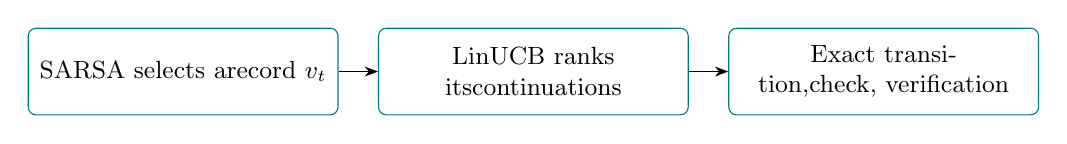
\begin{tikzpicture}[node distance=3mm and 5mm, every node/.style={font=\small,align=center},box/.style={draw=accent,rounded corners=1mm,minimum height=11mm,text width=37mm},>=Stealth]
\node[box] (a) {SARSA selects a\frontier record $v_t$};
\node[box,right=of a] (b) {LinUCB ranks its\permitted continuations};
\node[box,right=of b] (c) {Exact transition,\resource check, verification};
\draw[->] (a)--(b);\draw[->] (b)--(c);
\end{tikzpicture}
\end{center}
Rewards favor successful low-resource construction and fewer search allocations. Intermediate progress also supplies feedback.
\takeaway{The learner changes the order of exploration. It cannot declare a wrong circuit correct or override a proved resource restriction.}
\src{Return and action-value terminology: Sutton--Barto [SB]. Current native and cleanup search controllers: [N, L]. One search allocation may emit a verified multi-gate operation; its full physical cost is counted.}
\end{frame}

% 6
\begin{frame}[t]{6. SARSA learns which frontier record to try next}
\small
Let $x_t=x(S_t,v_t)$ contain small summaries of progress, resources, and remaining work. Use a linear action-value estimate:
\[
 \widehat q_w(S_t,v_t)=w^{\mathsf T}x_t.
\]
The temporal-difference error uses the \emph{next record actually selected}:
\[
 \delta_t=R_{t+1}+w_t^{\mathsf T}x_{t+1}-w_t^{\mathsf T}x_t.
\]
At termination the next value is zero. The implemented normalized update is
\[
 w_{t+1}=\Pi_{[-20,20]^d}\!\left(
 w_t+\frac{\alpha\,\delta_t x_t}{\max(1,\|x_t\|^2)}\right).
\]
Here $d$ is the feature count; $\Pi$ clips each coefficient to the displayed interval.
\takeaway{A positive $\delta_t$ says the observed continuation was better than predicted. During circuit-generation tests, the learned coefficients are fixed. Completing training does not prove convergence.}
\src{SARSA temporal-difference rule: [SB]. Normalization and coefficient bounds are implementation choices, not a convergence theorem: native\_policy.py and cleanup/policy.py [N, L].}
\end{frame}

% 7
\begin{frame}[t]{7. LinUCB ranks the eligible next operations}
\small
For each operation family $f$, let $z$ be its context and $y$ the recorded training feedback. A public prior $\beta_0$ is corrected by a small linear model:
\[
 A_f=I+\sum z z^{\mathsf T},\qquad
 b_f=\sum z\bigl(y-z^{\mathsf T}\beta_0\bigr),\qquad
 \widehat\beta_f=\beta_0+A_f^{-1}b_f.
\]
Rank the eligible operations by
\[
 \underbrace{z^{\mathsf T}\widehat\beta_f}_{\text{estimated value}}
 +\underbrace{\kappa\sqrt{z^{\mathsf T}A_f^{-1}z}}_{\text{training exploration}}.
\]
The feedback uses the reward and frontier-value information. Exploration is turned off and coefficients are fixed in evaluation.
\takeaway{In the current oracle method, exact algebra constructs the main candidates. SARSA--LinUCB is an \textbf{optional search for full-bank schedules}; it does not choose the deterministic factorization or exact lifetime order.}
\src{Disjoint linear models and actual role: cleanup/policy.py and cleanup/consumer\_search.py [L, C]. Families mean native gate types in native search, or permitted protocol operations in cleanup search. No general bandit regret claim is made.}
\end{frame}

% ======================= PAGES 8--11 ======================
\renewcommand{\partnamebar}{Measurement, cleanup theorem, and construction}
% 8
\begin{frame}[t]{8. Measurement erases a value only after its phase is corrected}
\small
A temporary value $f(z)$ is entangled with the input: $\sum_z\alpha_z\ket z\ket{f(z)}$.
For $s\in\{0,1\}$, define $\ket{s_X}=(\ket0+(-1)^s\ket1)/\sqrt2$. Then
\[
 \bra{s_X}f(z)\rangle=2^{-1/2}(-1)^{sf(z)}.
\]
After measurement, apply $D_f^s\ket z=(-1)^{sf(z)}\ket z$ and reset the measured qubit:
\[
 (-1)^{sf(z)}(-1)^{sf(z)}=1
 \quad\Longrightarrow\quad
 K_sJ_A=2^{-1/2}J_AO_p.
\]
An existing oracle sign $(-1)^{p(z)}$ is unchanged. Each outcome has probability $1/2$.

\labeltext{Useful case.} If $f=uv$, the correction is $\CZ_{u,v}^{\,s}$. A clean-target AND computes $uv$ with four T gates; its measured cleanup needs no more T gates.
\takeaway{The operand values needed for correction must remain available. A full measured circuit needs the coherent records \emph{plus} outcomes and correction dependencies; it is not one unitary tableau-and-rotation word.}
\src{Established temporary-AND and measured-termination constructions: Gidney [G], Amy--Ross [AR]. The native clean-input primitive and every correction are checked in this work [D, N].}
\end{frame}

% 9
\begin{frame}[t]{9. The theorem: a workspace optimum for a required full bank}
\fontsize{9.8}{11.5}\selectfont
Let independent inputs be $a\in\F$, $b\in\F^r$, $x\in\F^m$, and $F_{ij}=ab_ix_j$.
All $rm$ product qubits must coexist. The $k$ retained helpers have the form
\[
 H=a(Pb\oplus Qx\oplus c).
\]
Process $F$ alone; apply Clifford feedback preserving the live values; finally measure $H$ in $X$ and correct on the original inputs. Require exact deterministic cleanup.
\[
 \boxed{A_{\mathrm{peak}}^{\mathrm{full\ bank}}=rm+\min(r,m).}
\]
\begin{columns}[T,onlytextwidth]
\begin{column}{.47\textwidth}
\labeltext{Upper bound.} If $m\le r$, retain $H_j=ax_j$ and compute $F_{ij}=b_iH_j$. Measure $F$ and correct with CZs; then do the same for $H$. The other case is symmetric.
\end{column}
\begin{column}{.50\textwidth}
\labeltext{Lower-bound idea.} If $k<\min(r,m)$, take $b_0\ne0$ in $\ker P$. The proof uses the labels $(b_0,b_0\otimes x)$ for $x\in\ker Q$. At least $2^{m-k}>1$ labels are indistinguishable by permitted feedback. Measurement completeness gives $P_{\rm success}\le2^{-(m-k)}<1$.
\end{column}
\end{columns}
\takeaway{This is an optimum only for the stated full-bank architecture. A circuit implementing the final phase may avoid that bank entirely.}
\src{Supplied cleanup theorem, pp. 53--60 [H]. The lower-bound proof temporarily adds $h=ab$ as a proof device, not as construction workspace. Full assumptions and the reduction back to $F$ alone are in NOTES.md.}
\end{frame}

% 10
\begin{frame}[t]{10. The final phase can require far less stored information}
\fontsize{10}{12}\selectfont
The consumer is $p=q(a,b,x,F)$, where $q$ is quadratic in its displayed variables. Substitute $F_{ij}=ab_ix_j$ \emph{before} building the circuit. Exact binary factorization gives
\[
 p=q_0\oplus aB(b)^{\mathsf T}MX(x)
   =q_0\oplus\bigoplus_{\ell=1}^{d}aL_\ell(b)R_\ell(x),
 \qquad d=\operatorname{rank}_{\F}M.
\]
Here $q_0$ is quadratic; $B,X$ list linear and quadratic operand features.

For one factor, form $L,R$, use a clean $t$, and restore the parity wires afterward:
\[
 \ket{a,L,R,0}\xrightarrow{\AND(a,L;t)}\ket{a,L,R,aL}
 \xrightarrow{\CZ(t,R)}(-1)^{aLR}\ket{a,L,R,aL}.
\]
Measure $t$ in $X$ and correct with $\CZ(a,L)^s$. Slide 8 proves the branch is correct.
If $s_{\!f}$ distinct quadratic products are stored, this construction has
\[
 \boxed{N_T=4(d+s_{\!f}),\qquad A_{\mathrm{peak}}\le s_{\!f}+1.}
\]
\labeltext{Reason.} Each stored product and each factor uses one four-T AND; one factor helper is reused. Rank is minimal only in the chosen feature basis, not over all circuits.
\src{Exact factor construction and complete branch proof: [C, D]. Parity CNOTs, restoration, measurement and corrections are included in the measured resources. This is not the former fixed phase-polynomial search.}
\end{frame}

% 11
\begin{frame}[t]{11. Prepare at first use; erase after last use}
\fontsize{10}{12}\selectfont
Fix the factorization. Let $S_j$ be the temporary features needed by factor $j$, and let $A$ be the set of factors already completed. With no recomputation,
\[
 L(A)=\left(\bigcup_{i\in A}S_i\right)\cap
      \left(\bigcup_{i\notin A}S_i\right),
 \qquad w(A,j)=1+|L(A)\cup S_j|.
\]
The exact minimum peak within these orders is obtained by
\[
 V(A)=\min_{j\notin A}\max\{w(A,j),V(A\cup\{j\})\},
 \qquad V(\{1,\ldots,d\})=0.
\]
\labeltext{Why exact?} Every feature in $L(A)$ must remain for a future use; all of $S_j$ must exist during $j$. First-use preparation and last-use cleanup attain that bound.

\smallskip
Example: $S_1=S_3=\{A,D\}$, $S_2=S_4=\{B,C\}$.
\[
 (1,2,3,4):\ A_{\mathrm{peak}}=5
 \quad\longrightarrow\quad
 (1,3,2,4):\ A_{\mathrm{peak}}=3,
 \qquad N_T=32\ \text{in both}.
\]
\src{Quantum construction: [C, D]. The ordering is an application of minimum-open-stacks dynamic programming [MOS], not a new scheduling algorithm. Factors run sequentially; no feature compression or recomputation. Exact subset ordering is limited to $d\le16$.}
\end{frame}

% ======================= PAGES 12--15 =====================
\renewcommand{\partnamebar}{Results and conclusion}
% 12
\begin{frame}[t]{12. What was compared, and how resources were counted}
\fontsize{10}{12}\selectfont
\textbf{41 phase oracles:} five development examples and 36 additional synthetic functions. Each comparison uses the \emph{same final Boolean phase}.

\smallskip
\textbf{Current method:} deterministic full-bank, bank-free and factor constructions.\par
\textbf{Control:} authors' mockturtle XOR--AND optimization, followed by our measured-oracle construction using the same four-T AND and Clifford corrections.
\begin{center}
\begin{tabular}{@{}ll@{}}
\toprule
$N_T$ & T and T-dagger gates.\\
$A_{\mathrm{peak}}$ & Maximum simultaneously needed clean-origin ancillas; inputs excluded.\\
$N_{\mathrm{CNOT}},\ N_G$ & CNOT count and total native unitary gates, including corrections.\\
$\Lambda$ & Worst-case schedule: gate 1, measurement 5, outcome delay 2 ticks.\\
$R_m$ & Measurement stages in the emitted protocol.\\
\bottomrule
\end{tabular}
\end{center}
Both select by $(N_T,A_{\mathrm{peak}},\Lambda,N_G,N_{\mathrm{CNOT}})$: T-count first. These are \textbf{not} equal-workspace-cap optima. All reported protocols passed archived exact checks.
\src{Archived comparison [D], 41 targets x 2 methods x 3 repetitions = 246 records; repetitions are not independent functions. Current figures were not produced by RL. Timing is illustrative and all-to-all, not hardware data.}
\end{frame}

% 13
\begin{frame}[t]{13. Five development examples: all six resources}
\small
Each cell is \textbf{current / measured XOR--AND control}; lower is better.
\begin{center}
\setlength{\tabcolsep}{5pt}
\renewcommand{\arraystretch}{1.16}
\begin{tabular}{@{}lrrrrrr@{}}
\toprule
Shape & $N_T$ & $A_{\mathrm{peak}}$ & $N_{\mathrm{CNOT}}$ & $N_G$ & $\Lambda$ & $R_m$\\
\midrule
$3\!\times\!1$ & 8 / 8 & 2 / 2 & 21 / 21 & 51 / 51 & 58 / 36 & 2 / 1\\
$4\!\times\!2$ & 8 / 8 & 1 / 2 & 11 / 13 & 45 / 43 & 59 / 32 & 2 / 1\\
$5\!\times\!2$ & 12 / 16 & 2 / 4 & 22 / 29 & 68 / 87 & 79 / 68 & 3 / 2\\
$6\!\times\!3$ & 36 / 52 & 4 / 13 & 83 / 151 & 219 / 335 & 213 / 187 & 7 / 3\\
$8\!\times\!3$ & 56 / 64 & 5 / 16 & 120 / 169 & 324 / 395 & 248 / 186 & 8 / 3\\
\bottomrule
\end{tabular}
\end{center}
\labeltext{A concrete explanation: the $4\times2$ case.}
\[
 p=ax_2\oplus ab_2x_1\oplus ab_3x_2.
\]
The current circuit uses one helper twice, with cleanup after each use. The control keeps two products and cleans them together.
\takeaway{Both use eight T gates. Reusing a qubit changes $(A_{\mathrm{peak}},R_m,\Lambda)$ from $(2,1,32)$ to $(1,2,59)$: less workspace, but more waiting.}
\src{Source [D], original presentation pp. 34--35; exact final predicate and complete corrected circuits, not estimated counts. The shape labels describe source banks, which the selected circuit need not materialize.}
\end{frame}

% 14
\begin{frame}[t]{14. Across 36 additional oracles, workspace is the strength}
\small
Number of targets on which the current method is better, equal, or worse:
\begin{center}
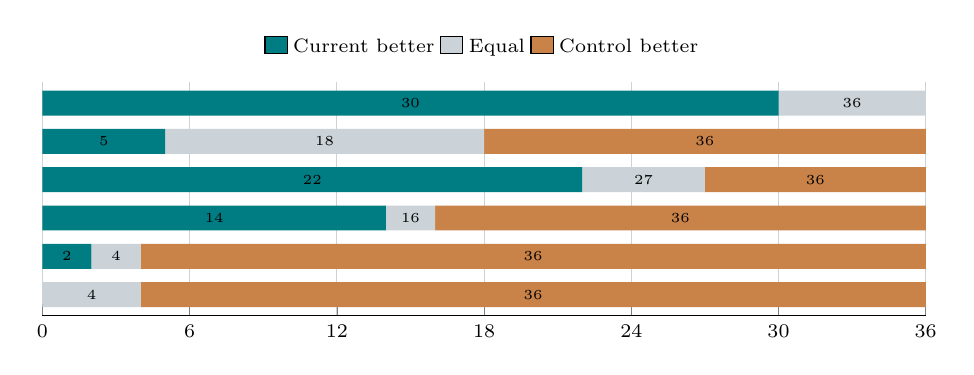
\begin{tikzpicture}
\begin{axis}[
 width=12.8cm,height=4.55cm,xbar stacked,bar width=9pt,
 xmin=0,xmax=36,xtick={0,6,12,18,24,30,36},
 ytick={0,1,2,3,4,5},
 yticklabels={Measurement rounds,Latency,Native gates,CNOTs,T-count,Clean ancillas},
 ymin=-.55,ymax=5.55,
 axis y line=none,axis x line*=bottom,
 tick label style={font=\scriptsize},label style={font=\scriptsize},
 xmajorgrids=true,grid style={draw=equal},
 legend style={at={(.5,1.06)},anchor=south,legend columns=3,draw=none,font=\scriptsize},
 nodes near coords,point meta=x,nodes near coords style={font=\tiny},
 enlarge y limits=false]
\addplot[fill=accent,draw=none] coordinates {(0,0)(2,1)(14,2)(22,3)(5,4)(30,5)};
\addplot[fill=equal,draw=none] coordinates {(4,0)(2,1)(2,2)(5,3)(13,4)(6,5)};
\addplot[fill=control,draw=none] coordinates {(32,0)(32,1)(20,2)(9,3)(18,4)(0,5)};
\legend{Current better,Equal,Control better}
\end{axis}
\end{tikzpicture}
\end{center}
\vspace{-2mm}
\takeaway{Ancillas improve on 30 targets and tie on 6. T-count is worse on 18; latency is worse on 32. These are resource trade-offs, not uniform superiority.}
\src{Archived exact resource vectors [D], original presentation pp. 39--44. Twelve bilinear, twelve quadratic-feature, twelve mixed-consumer functions. The control was not given the best possible space-constrained recomputation schedule.}
\end{frame}

% 15
\begin{frame}[t]{15. The result and the role of learning}
\small
\labeltext{What is proved.}\par
The corrected branches preserve the phase and return ancillas to zero. The full-bank theorem has a matching workspace bound. Fixed-factor ordering is exact only within its stated no-recomputation model.

\medskip
\labeltext{What the circuits show.}\par
Exact algebra and reuse of temporary values can reduce clean ancillas. The complete circuit may then need more T gates or more measurement time than an alternative.

\medskip
\labeltext{What reinforcement learning contributes so far.}\par
SARSA selects frontier records; LinUCB ranks allowed continuations. Both remain available, but the current benchmark improvements come from deterministic constructions. A learned advantage has not been established.
\takeaway{\textbf{Defensible claim:} certified synthesis for a specified family of Boolean phase oracles, with useful workspace--T-count--latency trade-offs. Not global ancilla optimality, not a complete BNN-verification speedup, and not SARSA--LinUCB superiority.}
\src{Next comparison: impose the same clean-ancilla and latency caps, allowing both methods to schedule and recompute. Full references, theorem assumptions, data provenance and mathematical notes are in NOTES.md.}
\end{frame}
\end{document}
